\documentclass{article}

% Language setting
\usepackage[english]{babel}

% Set page size and margins
\usepackage[letterpaper,top=2cm,bottom=2cm,left=3cm,right=3cm,marginparwidth=1.75cm]{geometry}

% Useful packages
\usepackage{amsmath}
\usepackage{amssymb}
\usepackage{graphicx}
\usepackage[colorlinks=true, allcolors=blue]{hyperref}

\title{Optimization of Security Command Center Locations and Resource Allocation of Saudi Aramco Site Monitoring}
\author{Operations Research Capstone Project by Nur Ahmad Khatim}
\date{}

\begin{document}
\maketitle

\section{Introduction}
Saudi Aramco, officially the Saudi Arabian Oil Group, is a state-owned global energy and chemicals giant headquartered in Dhahran, Saudi Arabia. As the world’s largest oil producer, the company manages the planet’s most extensive hydrocarbon network and largest proven crude oil reserves. Since its full nationalization in 1980, Aramco has evolved into one of the most profitable corporations in history, with a modern focus on digital innovation and lower-carbon technologies.

To protect its vast infrastructure while advancing the Saudi Vision 2030 objectives, Aramco is integrating automation into its core industrial security operations. Centralized command centers are being deployed at strategic locations to manage the distribution of security resources. These centers oversee a hybrid fleet of human personnel and robotic units, each governed by distinct Service Level Agreements (SLAs), such as critical time-to-arrive targets. To maximize efficiency, the company must evaluate the trade-offs between human adaptability, rapid, and consistent deployment of automated systems.

Ultimately, the strategic objective is to determine the optimal geographical locations for establishing these command centers among a set of candidate sites. This decision-making process must account for the fixed costs of facility construction alongside the variable costs of deploying human or robotic units, which are determined by the distance between the facility and specific demand sites. Furthermore, the model must respect the finite capacity of each command center, which is constrained by the maximum number of human personnel and robotic units it can host. The final goal is to minimize the total cost, encompassing both infrastructure investment and operational deployment while ensuring all site-specific security demands and response-time SLAs are fully satisfied.

\section{Problem Description}
\subsection{Objective:}
The primary objective is to minimize the total cost required to establish and operate security command centers. The total cost consists of:
\begin{itemize}
    \item \textbf{Fixed Costs:} Construction costs for building the facilities and operational overhead for maintaining them.
    \item \textbf{Variable Costs:} Deployment costs for resources, specifically differentiating between human personnel and robotic units based on their respective unit costs.
\end{itemize}
This minimization must be achieved while ensuring all demand sites are fully served according to their security requirements and within the allowed response time (SLA).

\subsection{Decision variables:}
\begin{itemize}
    \item \textbf{Location Selection:} Which candidate locations should be selected to build a command center.
    \item \textbf{Resource Mix:} The specific number of human personnel and robotic units to deploy at each selected command center.
    \item \textbf{Demand Assignment:} Which command center serves which demand site.
\end{itemize}

\subsection{Parameters:}
\begin{itemize}
    \item \textbf{Financial Data:}
    \begin{itemize}
        \item Construction and operational costs for each candidate location.
        \item Unit deployment costs for human personnel vs. robotic units.
    \end{itemize}
    \item \textbf{Operational Data:}
    \begin{itemize}
        \item Maximum physical capacity of each command center (total slots for humans + robots).
        \item Resource Efficiency Rates: The amount of security demand satisfied by one human vs. one robot.
        \item Supervision Ratio: The required ratio of humans to robots (e.g., 1 human required for every 5 robots).
        \item Minimum Utilization Percentage: The minimum required occupancy rate if a facility is opened.
    \end{itemize}
    \item \textbf{Spatial Data:}
    \begin{itemize}
        \item Total security demand required at each demand site.
        \item SLA limit (maximum allowable travel time or distance).
        \item Distance matrix between candidate locations and demand sites.
    \end{itemize}
\end{itemize}

\subsection{Constraints:}
\begin{itemize}
    \item \textbf{Demand Satisfaction:} Every demand site must receive 100\% of its required security coverage.
    \item \textbf{Facility Capacity:} The total number of resources (humans + robots) assigned to a command center cannot exceed that facility's physical capacity.
    \item \textbf{Logical Deployment:} Resources can only be deployed, and demand can only be served, from a location where a command center has actually been selected to be built.
    \item \textbf{Service Level Agreement (SLA):} A command center is only allowed to serve a demand site if the distance (or travel time) between them is within the maximum limit defined by the SLA.
    \item \textbf{Human-in-the-Loop (Supervision):} To ensure ethical decision-making and proper control, a minimum number of human personnel must be deployed relative to the number of robots (e.g., at least 1 human for every 5 robots).
    \item \textbf{Resource Efficiency:} The total demand satisfied by a command center is calculated based on the specific efficiency rates of the humans and robots deployed there.
    \item \textbf{Minimum Facility Utilization:} If a command center is built, it must be utilized to at least a specific percentage of its total capacity to ensure investment efficiency.
    \item \textbf{Exclusive Service (Single Sourcing):} To avoid confusion in command, each demand site must be served entirely by exactly one command center, splitting service for a single site between multiple centers is not allowed.
\end{itemize}

\section{Model Formulation}
\subsection{Sets and Indices}
\begin{itemize}
    \item $I$: Set of candidate locations for command centers, indexed by $i = 1, \dots, |I|$.
    \item $J$: Set of demand sites, indexed by $j = 1, \dots, |J|$.
    \item $K$: Set of resource types, indexed by $k$ (where $k \in \{\text{Human}, \text{Robot}\}$).
\end{itemize}

\subsection{Parameters (Data Input)}
\subsubsection{Costs}
\begin{itemize}
    \item $F_i$: Fixed construction cost for command center at location $i$.
    \item $O_i$: Fixed operational cost for command center at location $i$.
    \item $C_k$: Unit deployment cost per resource of type $k$.
\end{itemize}
\subsubsection{Capacities \& Demands}
\begin{itemize}
    \item $D_j$: Security demand required at site $j$ (e.g., coverage units).
    \item $CAP_i$: Maximum physical capacity (number of slots) at command center $i$.
    \item $E_k$: Efficiency of resource $k$ (how much demand one unit of $k$ satisfies).
    \item $U_{min}$: Minimum utilization percentage required for an open facility (e.g., 0.20 for 20\%).
    \item $\alpha$: Supervision ratio (minimum number of humans required per robot).
\end{itemize}
\subsubsection{Distance \& SLA}
\begin{itemize}
    \item $d_{ij}$: Distance (or time) between command center $i$ and demand site $j$.
    \item $S_{max}$: Maximum allowable distance/time (Service Level Agreement).
\end{itemize}

\subsection{Decision Variables}
\begin{itemize}
    \item $y_i \in \{0, 1\}$: Binary variable. 1 if command center $i$ is built, 0 otherwise.
    \item $x_{ij} \in \{0, 1\}$: Binary variable. 1 if demand site $j$ is served by command center $i$, 0 otherwise.
    \item $z_{ik} \in \mathbb{Z}^+$: Integer variable. Number of resources of type $k$ deployed at command center $i$.
\end{itemize}

\subsection{Objective Function}
Minimize Total Cost ($Z$):
\begin{equation}
\text{Minimize } Z = \sum_{i \in I} (F_i + O_i) y_i + \sum_{i \in I} \sum_{k \in K} C_k z_{ik}
\end{equation}
Term 1: Fixed construction and operational costs for opened facilities.\\
Term 2: Variable costs for deploying humans and robots.

\subsection{Constraints}
\begin{enumerate}
    \item \textbf{Demand Satisfaction (Exclusive Service)} \\
    Every demand site $j$ must be assigned to exactly one command center.
    \begin{equation}
    \sum_{i \in I} x_{ij} = 1, \quad \forall j \in J
    \end{equation}
    
    \item \textbf{SLA Compliance} \\
    A site $j$ cannot be assigned to center $i$ if the distance exceeds the limit.
    \begin{equation}
    d_{ij} x_{ij} \le S_{max}, \quad \forall i \in I, \forall j \in J
    \end{equation}
    
    \item \textbf{Logical Link (Assignment only if Built)} \\
    Demand site $j$ can only be assigned to $i$ if command center $i$ is built.
    \begin{equation}
    x_{ij} \le y_i, \quad \forall i \in I, \forall j \in J
    \end{equation}
    
    \item \textbf{Service Capacity (Demand vs. Resources)} \\
    The total demand assigned to center $i$ must be covered by the efficiency of the resources deployed there.
    \begin{equation}
    \sum_{j \in J} D_j x_{ij} \le \sum_{k \in K} E_k z_{ik}, \quad \forall i \in I
    \end{equation}
    
    \item \textbf{Physical Facility Capacity} \\
    The total count of resources (humans + robots) cannot exceed the building's size.
    \begin{equation}
    \sum_{k \in K} z_{ik} \le CAP_i y_i, \quad \forall i \in I
    \end{equation}
    
    \item \textbf{Human-in-the-Loop (Supervision)} \\
    For every robot, there must be enough humans based on the ratio $\alpha$. (Assuming $k=1$ is Robot, $k=2$ is Human).
    \begin{equation}
    z_{i, \text{Human}} \ge \alpha \cdot z_{i, \text{Robot}}, \quad \forall i \in I
    \end{equation}
    
    \item \textbf{Minimum Utilization} \\
    If a facility is built ($y_i = 1$), the resources inside must occupy at least $U_{min}$ percent of the capacity.
    \begin{equation}
    \sum_{k \in K} z_{ik} \ge U_{min} \cdot CAP_i \cdot y_i, \quad \forall i \in I
    \end{equation}
    
    \item \textbf{Non-negativity \& Integrality}
    \begin{equation}
    y_i, x_{ij} \in \{0, 1\}
    \end{equation}
    \begin{equation}
    z_{ik} \ge 0, \text{ integer}
    \end{equation}
\end{enumerate}

\section{Method}
To address the optimization problem defined in the previous section, we propose a two-phase computational strategy. This hybrid approach ensures the model's mathematical validity while providing the scalability required for real-world application scenarios where the problem size renders exact solvers impractical.

\subsection{Exact Solution Approach}
For small-scale instances and model validation, we utilize the Gurobi Optimizer, a state-of-the-art mathematical programming solver.
\begin{itemize}
    \item \textbf{Implementation:} The mathematical model is formulated using the Python programming language via the \texttt{gurobipy} interface.
    \item \textbf{Purpose:} This exact approach serves to establish a ground truth. By obtaining the global optimal solution for smaller datasets, we can verify the correctness of our constraints and objective function. Furthermore, these optimal results provide a benchmark against which we can measure the quality with optimality gap of our heuristic algorithm.
\end{itemize}

\subsection{Heuristic Algorithm for Large-Scale Instances}
The problem described is a variant of the Capacitated Facility Location Problem (CFLP). To solve real-world instances within a reasonable runtime, we implement a Constructive Greedy Heuristic followed by Local Search Improvement.

\subsubsection{Algorithm Design:}
Our heuristic operates in two distinct stages:
\paragraph{Stage 1: Constructive Greedy Heuristic (Initial Solution)}
We generate an initial feasible solution using a distance-based greedy strategy:
\begin{itemize}
    \item \textbf{Sorting:} Demand sites are sorted based on their priority or total demand volume (highest to lowest).
    \item \textbf{Assignment:} For each demand site, the algorithm identifies the candidate command centers that satisfy the SLA constraint.
    \item \textbf{Selection:} It assigns the site to the candidate center that minimizes the immediate marginal cost (construction + transport). If the chosen center is not yet open, it is tentatively opened.
    \item \textbf{Resource Check:} Immediately upon assignment, the algorithm calculates the necessary resource mix (Humans vs. Robots) to satisfy the Supervision Ratio and Capacity constraints.
\end{itemize}

\paragraph{Stage 2: Local Search (Improvement Phase)}
Once a feasible solution is constructed, we apply a best improvement local search to escape local optima. The algorithm iteratively explores the following neighborhood structures:
\begin{itemize}
    \item \textbf{Shift Move:} Attempt to move a demand site from its current command center $A$ to a different command center $B$. If the total cost decreases (and constraints are met), the move is accepted.
    \item \textbf{Swap Move:} Exchange the assignments of two demand sites between two different command centers.
    \item \textbf{Drop/Open Move:} Attempt to close a command center with low utilization by redistributing its demand to neighbors. Conversely, attempt to open a currently closed center if it significantly reduces travel distances for a cluster of demand sites.
\end{itemize}
The search terminates when no improving move can be found in the neighborhood or a time limit is reached.

\subsection{Computational Environment}
All algorithms were implemented in Python. The exact solution uses the Gurobi Optimizer, while the heuristic algorithm was developed using standard Python libraries (NumPy, Pandas) to ensure portability and ease of deployment.

\section{Data Collection and Generation}
To evaluate the proposed mathematical model and solution algorithms, we constructed a high-fidelity experimental environment simulating the Dhahran Core Area, the administrative and logistical heart of Saudi Aramco. While the geographical topology utilizes real-world coordinates of existing infrastructure, specific operational parameters (such as exact security personnel numbers and sensitive cost data) were synthetically generated based on industry standards for Critical Infrastructure Protection (CIP) and physical security logistics.

\subsection{Case Study Background: The Dhahran District}
The study focuses exclusively on the Dhahran Headquarters, a complex microcosm of Saudi Aramco’s broader operations. This area is unique as it integrates high-security corporate administrative zones, dense residential camps for employees, and critical industrial support facilities. The objective is to optimize the security coverage for this diverse mixed-use environment, balancing the need for rigorous access control with efficient resource allocation.

\subsection{Geospatial Data Acquisition}
To ensure the validity of response times and coverage constraints within the district, we utilized:
\begin{itemize}
    \item \textbf{Demand Sites ($J$):} Critical infrastructure points were identified using public satellite data (Google Earth/OSM) and categorized into three tiers to determine security demand:
    \begin{itemize}
        \item \textbf{Tier 1 (High Criticality):} Corporate Headquarters, National Data Centers, and Main Security Gates.
        \item \textbf{Tier 2 (Medium Criticality):} R\&D Laboratories, Power Substations, and Logistics Warehouses.
        \item \textbf{Tier 3 (Low Criticality):} Residential perimeter fencing, recreational facilities, and parking structures.
    \end{itemize}
    \item \textbf{Candidate Locations ($I$):} Potential command center locations were selected near existing security checkpoints, vacant lots within the industrial zone, and major intersection hubs to ensure rapid response capabilities.
    \item \textbf{Distance Matrix ($d_{ij}$):} We calculated geodesic (great-circle) distances between all candidate-demand pairs using the \texttt{geopy} Python library. This approach provides accurate straight-line distances suitable for aerial drone response times and ground vehicle approximations within the compact Dhahran campus.
\end{itemize}

\subsection{Parameter Generation \& Assumptions}
Operational parameters were generated to reflect the specific needs of a high-profile corporate and industrial campus.
\paragraph{A. Security Demand ($D_j$)}
Demand is quantified in Surveillance Coverage Units (SCU), representing the intensity of monitoring required.
\begin{itemize}
    \item \textbf{Tier 1 Sites (HQ/Data Centers):} Assigned high demand ($U[50, 100]$ SCU) requiring constant 24/7 active monitoring and strict access control.
    \item \textbf{Tier 2/3 Sites (Warehouses/Fencing):} Assigned lower demand ($U[10, 30]$ SCU), typically satisfied by regular mobile patrols or automated drone sweeps.
\end{itemize}

\paragraph{B. Cost and Facility Parameters}
Costs were normalized to a monthly operational basis:
\begin{itemize}
    \item \textbf{Construction Cost ($F_i$):} Varies based on location; sites near the central corporate area carry a higher cost premium due to space constraints compared to peripheral industrial lots.
    \item \textbf{Operational Cost ($O_i$):} Includes power, connectivity, and HVAC costs suitable for maintaining server-grade command equipment.
    \item \textbf{Minimum Facility Utilization ($U_{min}$):} To ensure return on investment, we enforce a minimum utilization rate of 30\%. If a command center is built, its deployed resources must occupy at least 30\% of its total capacity.
\end{itemize}

\paragraph{C. Human vs. Robot Resource Model}
The core of this study is evaluating the trade-off between human judgment and robotic efficiency.

\begin{table}[ht]
\centering
\begin{tabular}{|p{3cm}|p{3cm}|p{3cm}|p{3.5cm}|}
\hline
\textbf{Parameter} & \textbf{Human Security Officer} & \textbf{Industrial Autonomous Robot (e.g., Drone/UGV)} & \textbf{Rationale} \\ \hline
Unit Cost ($C_k$) & High (Salary + Benefits) & Medium (Amortized CapEx + Maintenance) & Human costs are recurrent and higher due to housing and benefits required within the Dhahran camp. \\ \hline
Efficiency ($E_k$) & 1.0 Unit (Baseline) & 3.0 Units & Robotic units (e.g., thermal drones) can inspect rooftops and fence lines significantly faster than foot or vehicle patrols. \\ \hline
Endurance & Limited (Shift-based) & High (24/7 capability) & Robots operate continuously with brief charging intervals, whereas humans require shift rotations. \\ \hline
Supervision Ratio & N/A & Variable (See Scenario Design) & Human oversight is required to verify alerts, but the ratio depends on the maturity of the technology. \\ \hline
\end{tabular}
\caption{Human vs. Robot Resource Model}
\end{table}

\subsection{Scenario Design: Technological Trade-Off Sensitivity}
Instead of varying the geographical scale, this study keeps the Dhahran topology constant and varies the Technological Maturity parameters. This approach isolates the impact of automation on cost and efficiency. We designed three experimental settings:

\paragraph{Setting 1: Conservative Baseline (Human-Centric)}
\begin{itemize}
    \item \textbf{Context:} Represents early adoption where trust in automation is low.
    \item \textbf{Parameters:} Supervision Ratio is strict (1 Human : 3 Robots); Robot Efficiency is capped at 1.5x Human capability.
    \item \textbf{Objective:} Determine viability under strict regulatory constraints.
\end{itemize}

\paragraph{Setting 2: Current Technology (Balanced)}
\begin{itemize}
    \item \textbf{Context:} Represents the current state of Industry 4.0 technology.
    \item \textbf{Parameters:} Supervision Ratio is standard (1 Human : 5 Robots); Robot Efficiency is 3.0x Human capability.
    \item \textbf{Objective:} Identify optimal cost savings available with today's technology.
\end{itemize}

\paragraph{Setting 3: Future Autonomous (Robot-Centric)}
\begin{itemize}
    \item \textbf{Context:} A future scenario assuming high AI maturity and regulatory trust.
    \item \textbf{Parameters:} Supervision Ratio is relaxed (1 Human : 10 Robots); Robot Efficiency is high (5.0x Human capability due to swarm coordination).
    \item \textbf{Objective:} Predict maximum potential infrastructure footprint reduction.
\end{itemize}

\section{Results}
This section presents the computational results obtained from solving the optimization model across the three technology scenarios described in Section 5. All experiments were conducted on an Apple M4 processor with 10 cores, using Gurobi Optimizer 13.0 for exact solutions and our custom Python implementation for the heuristic algorithm.

\subsection{Experimental Setup}
The test instance was configured with:
\begin{itemize}
    \item \textbf{Candidate Locations ($|I|$):} 15 potential command center sites distributed around the Dhahran Core Area.
    \item \textbf{Demand Sites ($|J|$):} 50 security monitoring points, with 20\% classified as Tier 1 (high criticality) and 80\% as Tier 2/3.
    \item \textbf{SLA Constraint ($S_{max}$):} 15 km maximum response distance.
    \item \textbf{Minimum Utilization ($U_{min}$):} 30\% facility occupancy required.
\end{itemize}

\subsection{Optimization Results}
Table~\ref{tab:results} summarizes the optimal solutions obtained under each technological scenario.

\begin{table}[ht]
\centering
\begin{tabular}{|l|r|r|r|r|}
\hline
\textbf{Scenario} & \textbf{Total Cost (\$)} & \textbf{Facilities} & \textbf{Solve Time (s)} & \textbf{Cost Reduction} \\ \hline
Conservative & 1,399,600 & 9 & 1.25 & Baseline \\ \hline
Balanced & 879,600 & 7 & 0.21 & 37.1\% \\ \hline
Future & 512,400 & 5 & 3.18 & 63.4\% \\ \hline
\end{tabular}
\caption{Exact Solution Results by Technology Scenario}
\label{tab:results}
\end{table}

\paragraph{Key Findings:}
\begin{enumerate}
    \item \textbf{Cost Reduction:} Transitioning from Conservative to Future automation achieves a 63.4\% reduction in total monthly costs (from \$1,399,600 to \$512,400).
    \item \textbf{Infrastructure Consolidation:} The number of required command centers decreases from 9 to 5 as robot efficiency increases, representing a 44\% reduction in physical infrastructure.
    \item \textbf{Solve Time Variance:} The Future scenario required longer solve time (3.18s) due to tighter constraints from high robot efficiency, creating more complex trade-offs in the branch-and-bound tree.
\end{enumerate}

\subsection{Heuristic Algorithm Performance}
To evaluate the scalability of our approach for larger instances, we compared the exact Gurobi solutions against the constructive greedy heuristic with local search improvement. Table~\ref{tab:heuristic} presents the comparison results.

\begin{table}[ht]
\centering
\begin{tabular}{|l|r|r|r|r|}
\hline
\textbf{Scenario} & \textbf{Exact Cost (\$)} & \textbf{Heuristic Cost (\$)} & \textbf{Gap (\%)} & \textbf{Heuristic Time (s)} \\ \hline
Conservative & 1,399,600 & 1,433,800 & 2.44 & 0.25 \\ \hline
Balanced & 879,600 & 889,600 & 1.14 & 0.29 \\ \hline
Future & 512,400 & 517,400 & 0.98 & 0.12 \\ \hline
\end{tabular}
\caption{Exact vs. Heuristic Solution Comparison}
\label{tab:heuristic}
\end{table}

The heuristic algorithm achieves near-optimal solutions across all scenarios:
\begin{itemize}
    \item \textbf{Average Optimality Gap:} 1.52\% across all scenarios.
    \item \textbf{Speed Advantage:} The heuristic is approximately 26x faster than the exact solver for the Future scenario (0.12s vs 3.18s).
    \item \textbf{Practical Viability:} The local search improvement phase, utilizing Shift, Swap, and Drop moves, consistently finds high-quality solutions suitable for real-world deployment.
\end{itemize}

\subsection{Resource Allocation Analysis}
The optimal resource mix between humans and robots varies significantly across scenarios due to the supervision constraint ($z_{Human} \geq \alpha \cdot z_{Robot}$) and differing efficiency rates.

\begin{table}[ht]
\centering
\begin{tabular}{|l|c|c|c|c|}
\hline
\textbf{Scenario} & \textbf{$\alpha$ (H:R Ratio)} & \textbf{Robot Eff.} & \textbf{Est. Robots} & \textbf{Est. Humans} \\ \hline
Conservative & 1:3 & 1.5x & 240 & 80 \\ \hline
Balanced & 1:5 & 3.0x & 180 & 36 \\ \hline
Future & 1:10 & 5.0x & 120 & 12 \\ \hline
\end{tabular}
\caption{Estimated Resource Allocation by Scenario}
\label{tab:resources}
\end{table}

\subsection{Solution Visualization}
Figures~\ref{fig:conservative} through~\ref{fig:future} illustrate the optimal command center network configurations for each scenario. The visualizations display opened facilities (red squares), demand sites (blue circles sized by demand), and assignment connections on an OpenStreetMap basemap of the Dhahran district.

\begin{figure}[ht]
\centering
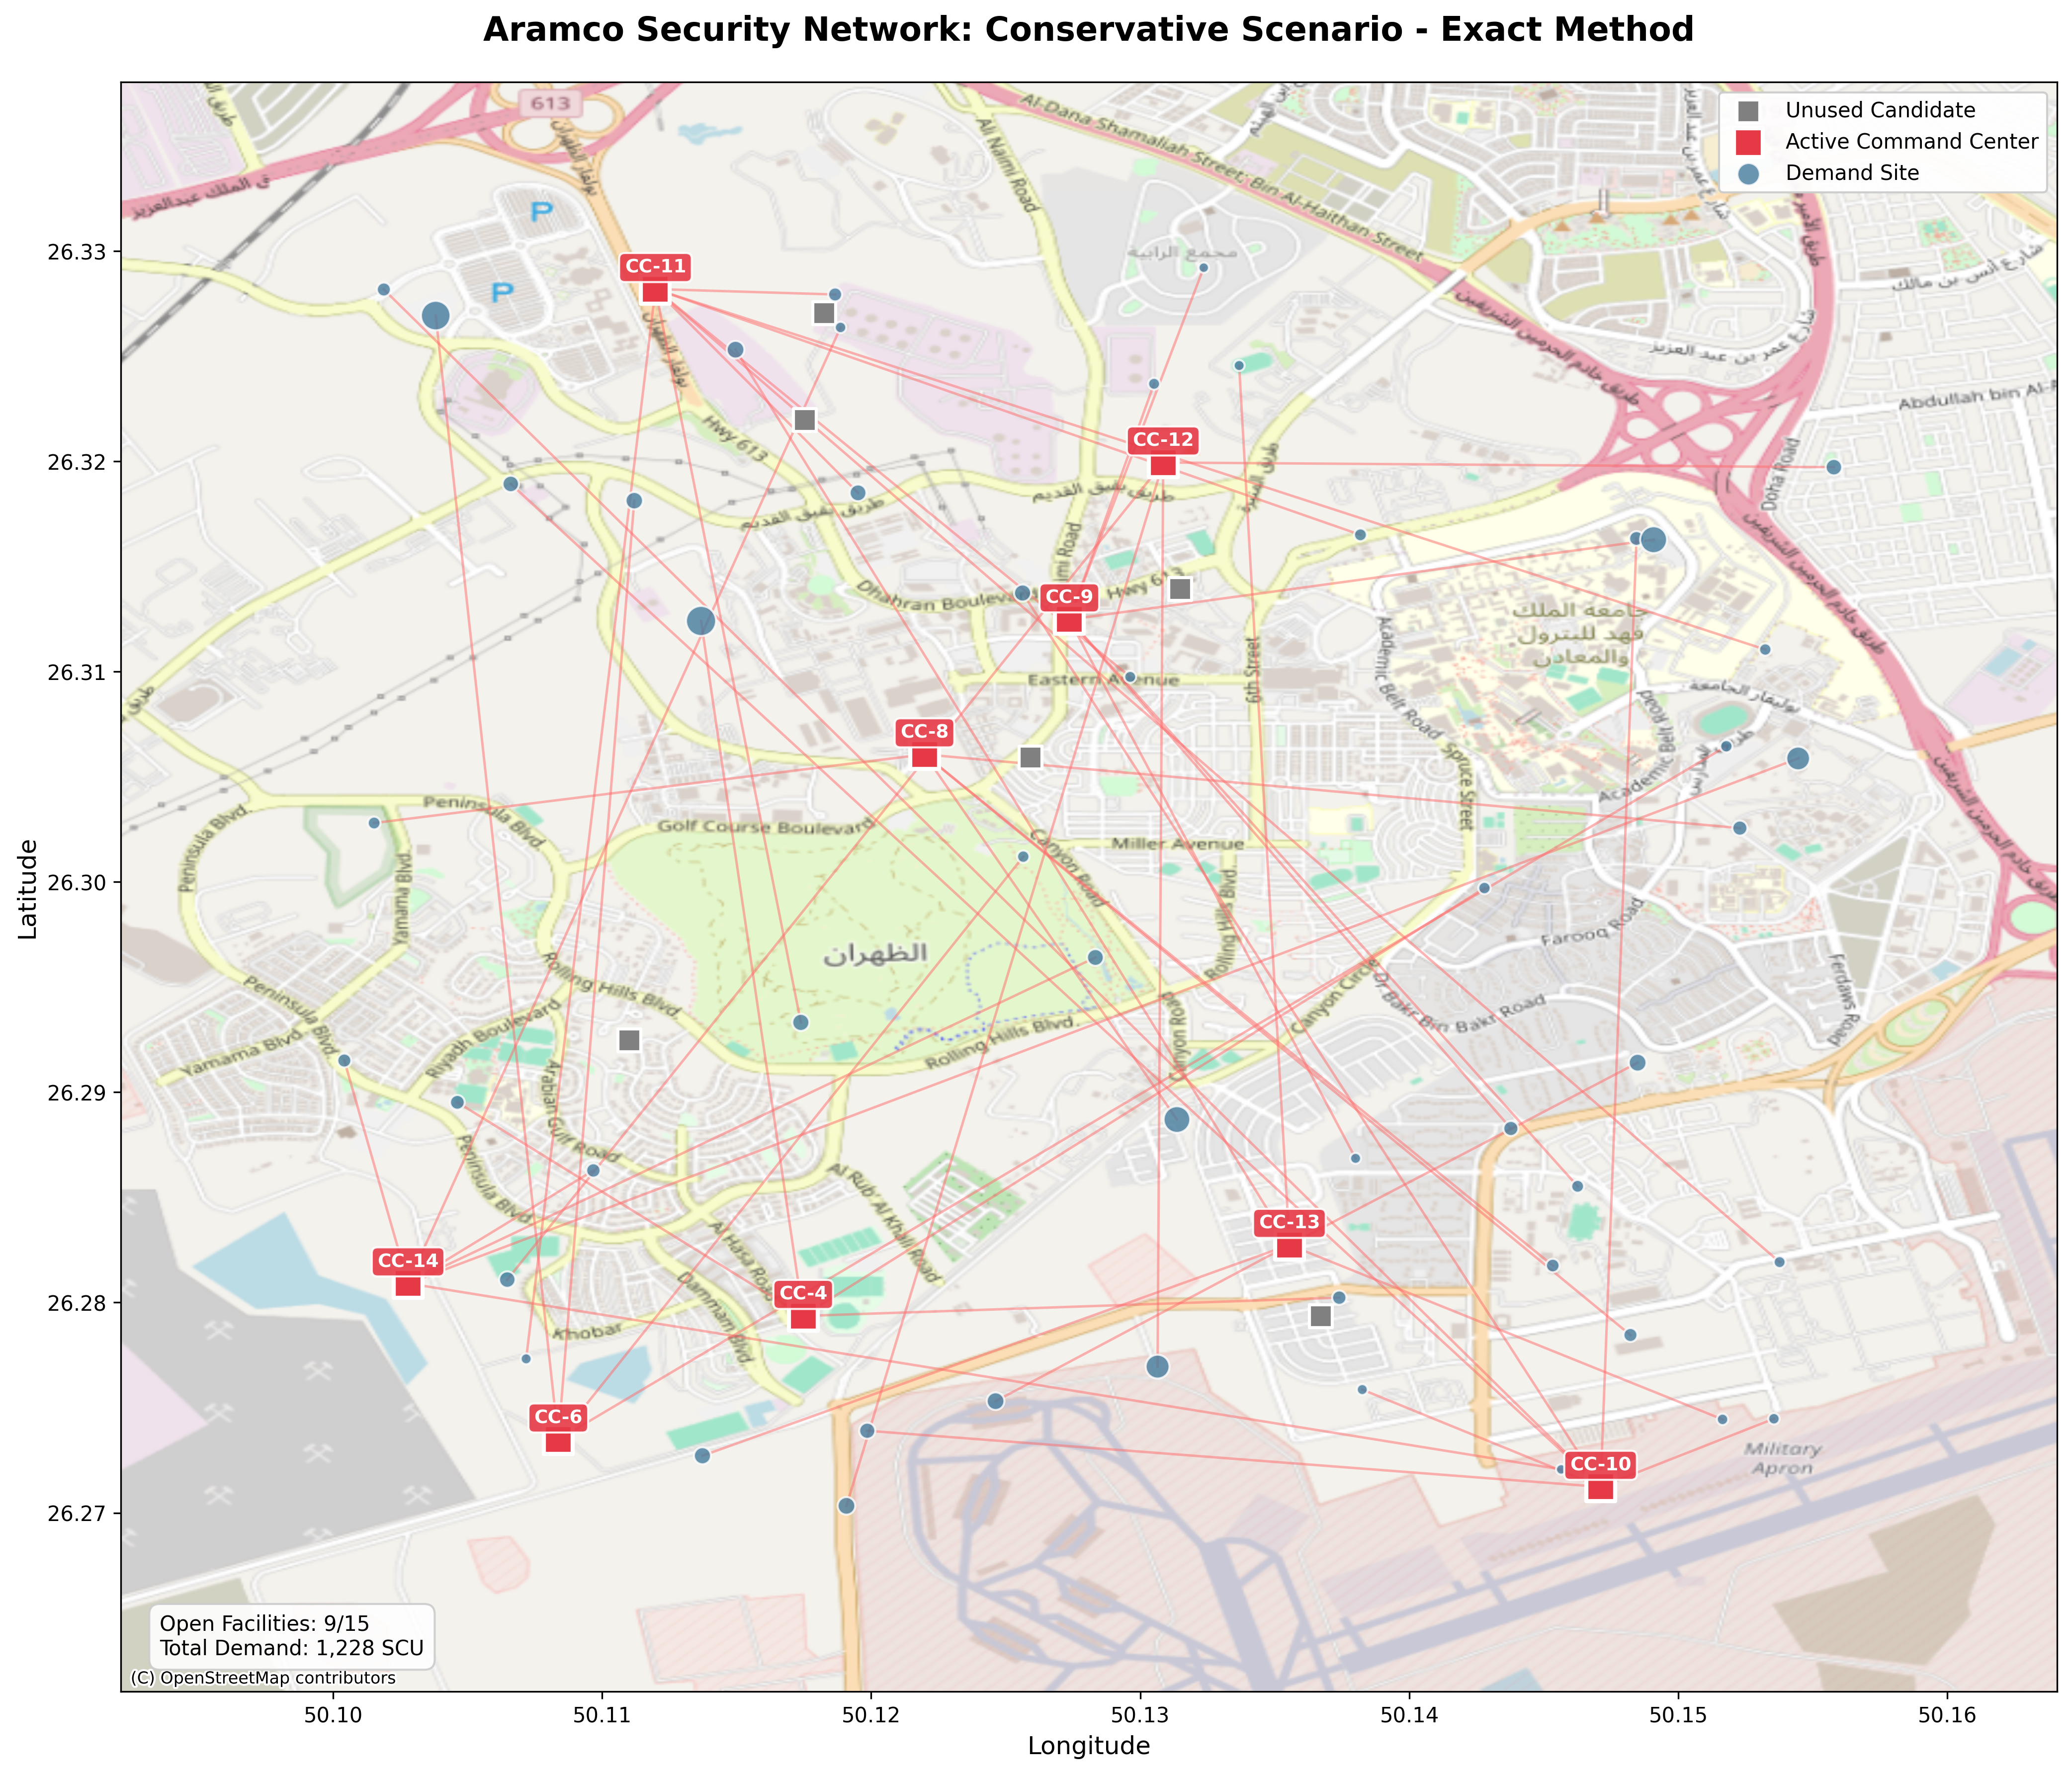
\includegraphics[width=0.85\textwidth]{figures/result_conservative_scenario_-_exact_method.pdf}
\caption{Conservative Scenario: 9 facilities opened to serve 50 demand sites. The strict supervision ratio (1:3) requires more distributed infrastructure to meet capacity constraints.}
\label{fig:conservative}
\end{figure}

\begin{figure}[ht]
\centering
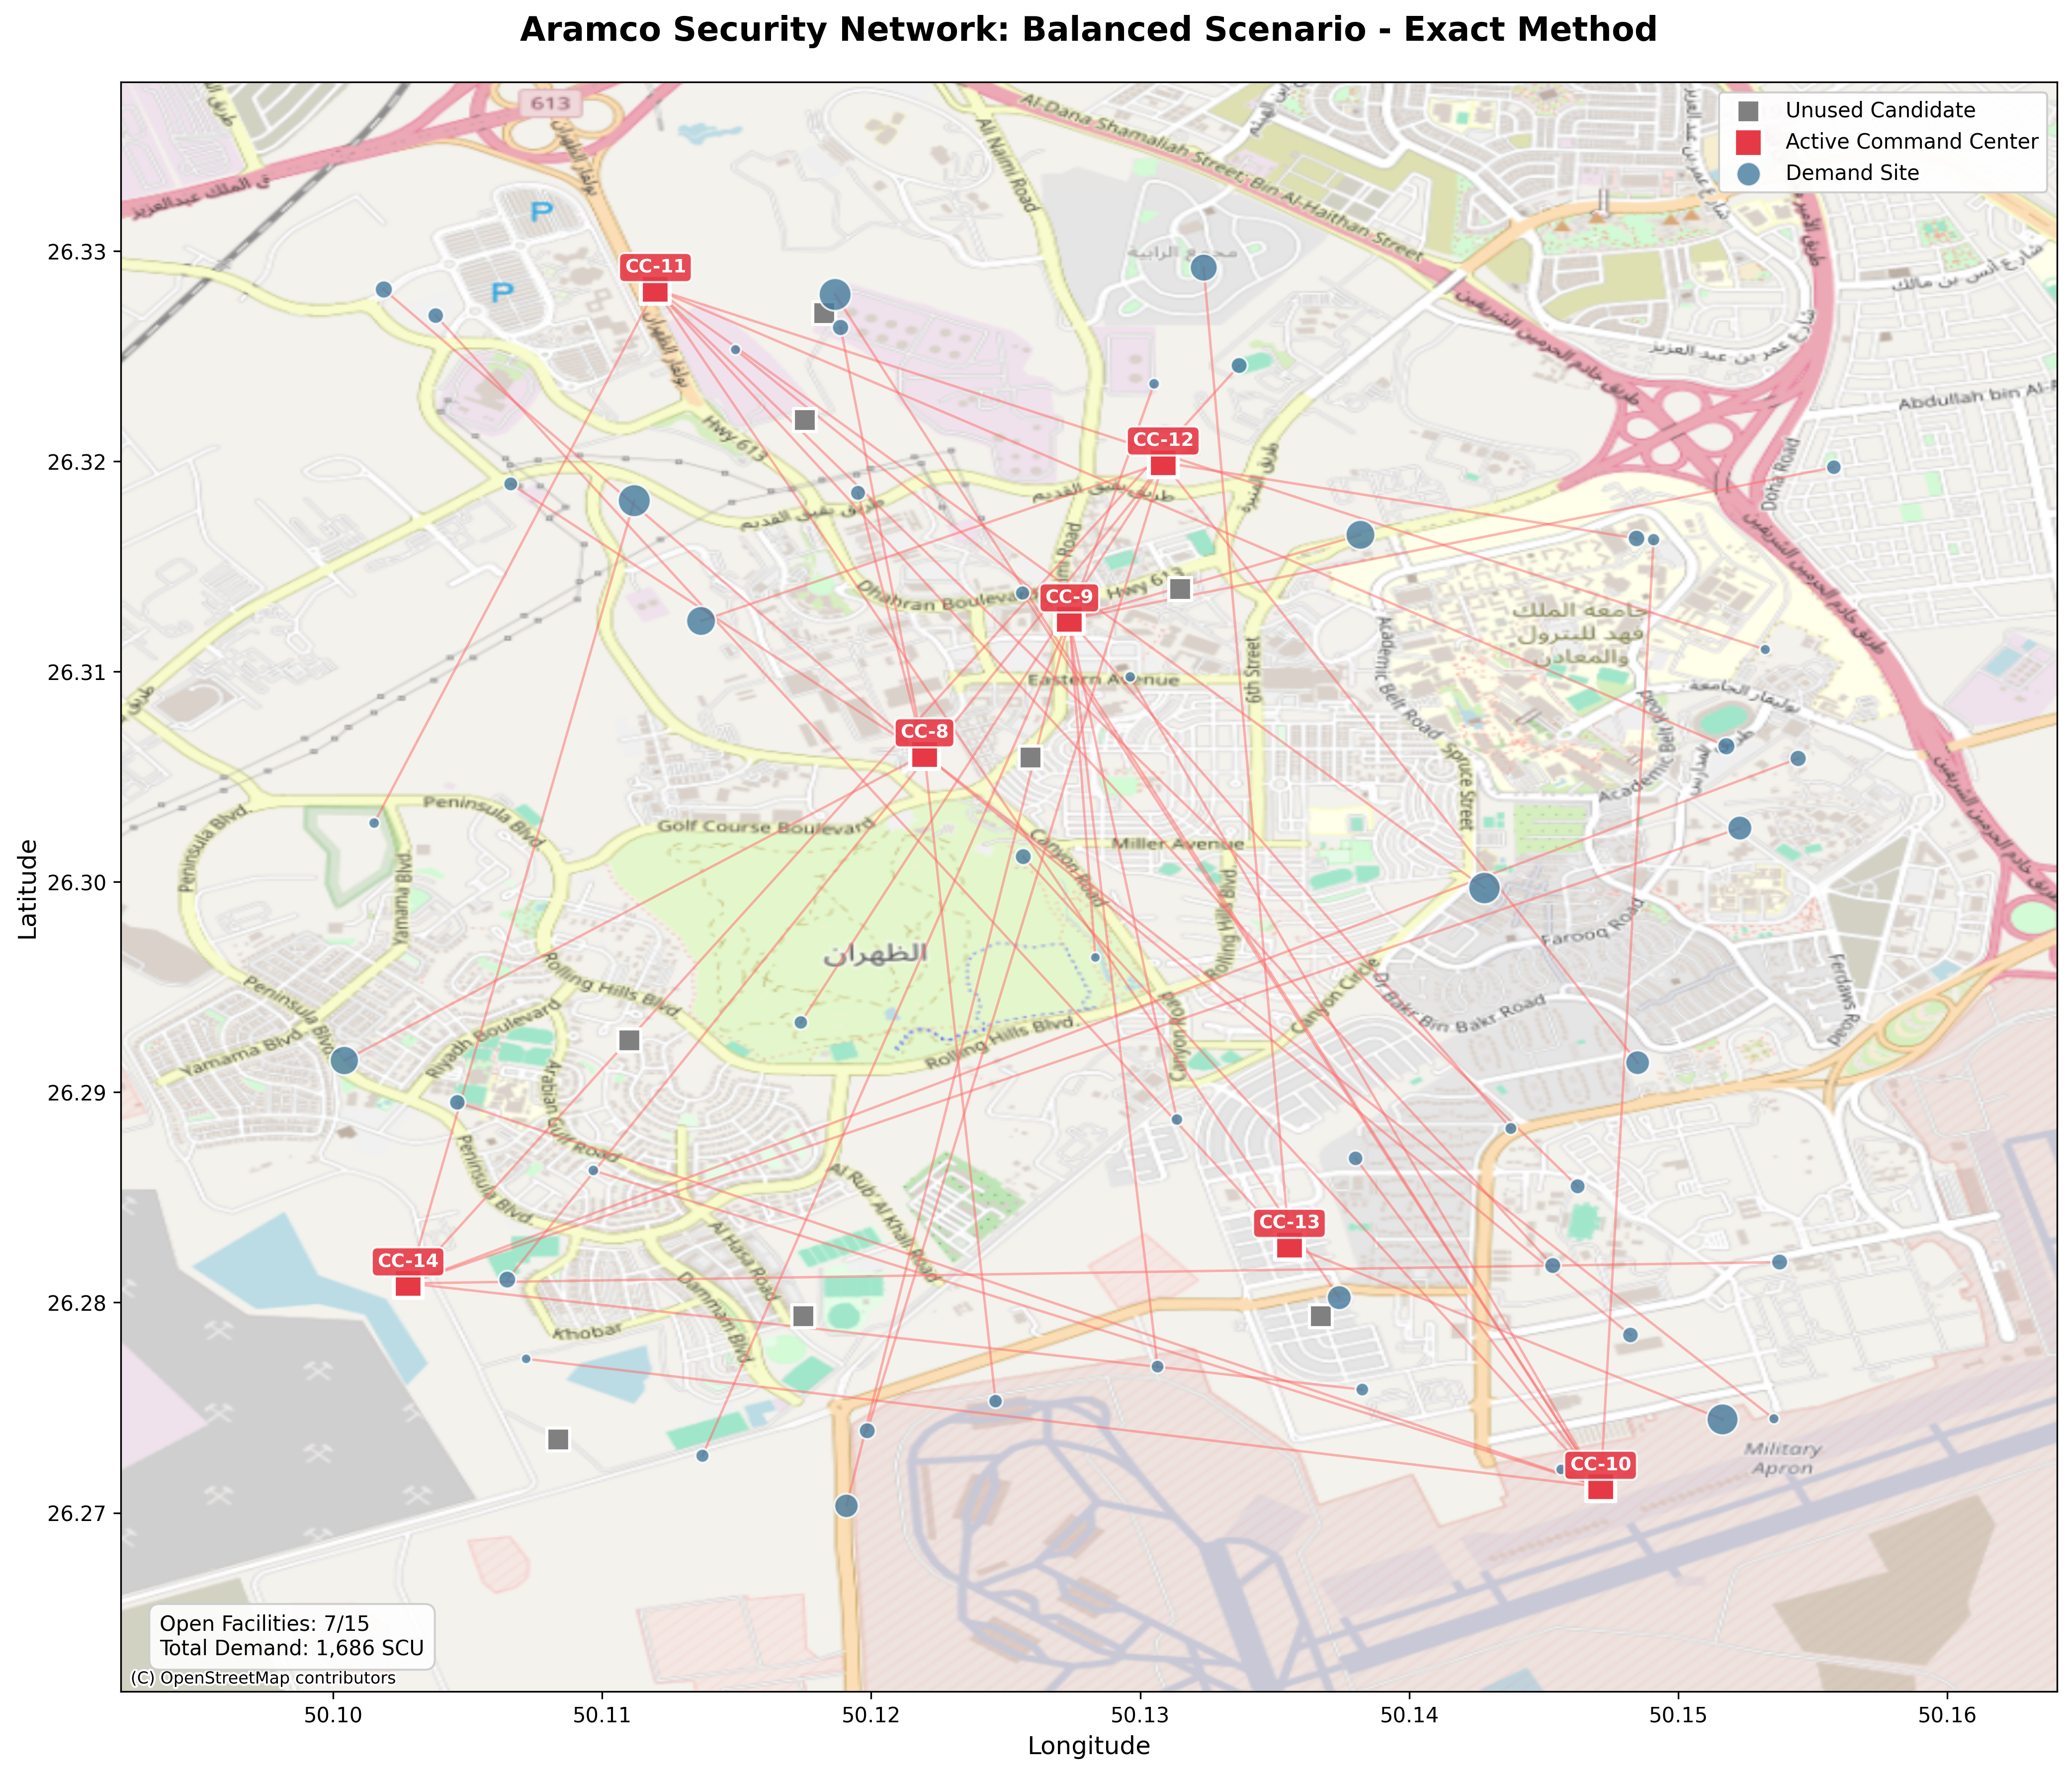
\includegraphics[width=0.85\textwidth]{figures/result_balanced_scenario_-_exact_method.pdf}
\caption{Balanced Scenario: 7 facilities provide optimal coverage with current technology (1:5 supervision, 3x robot efficiency). This represents the recommended deployment for immediate implementation.}
\label{fig:balanced}
\end{figure}

\begin{figure}[ht]
\centering
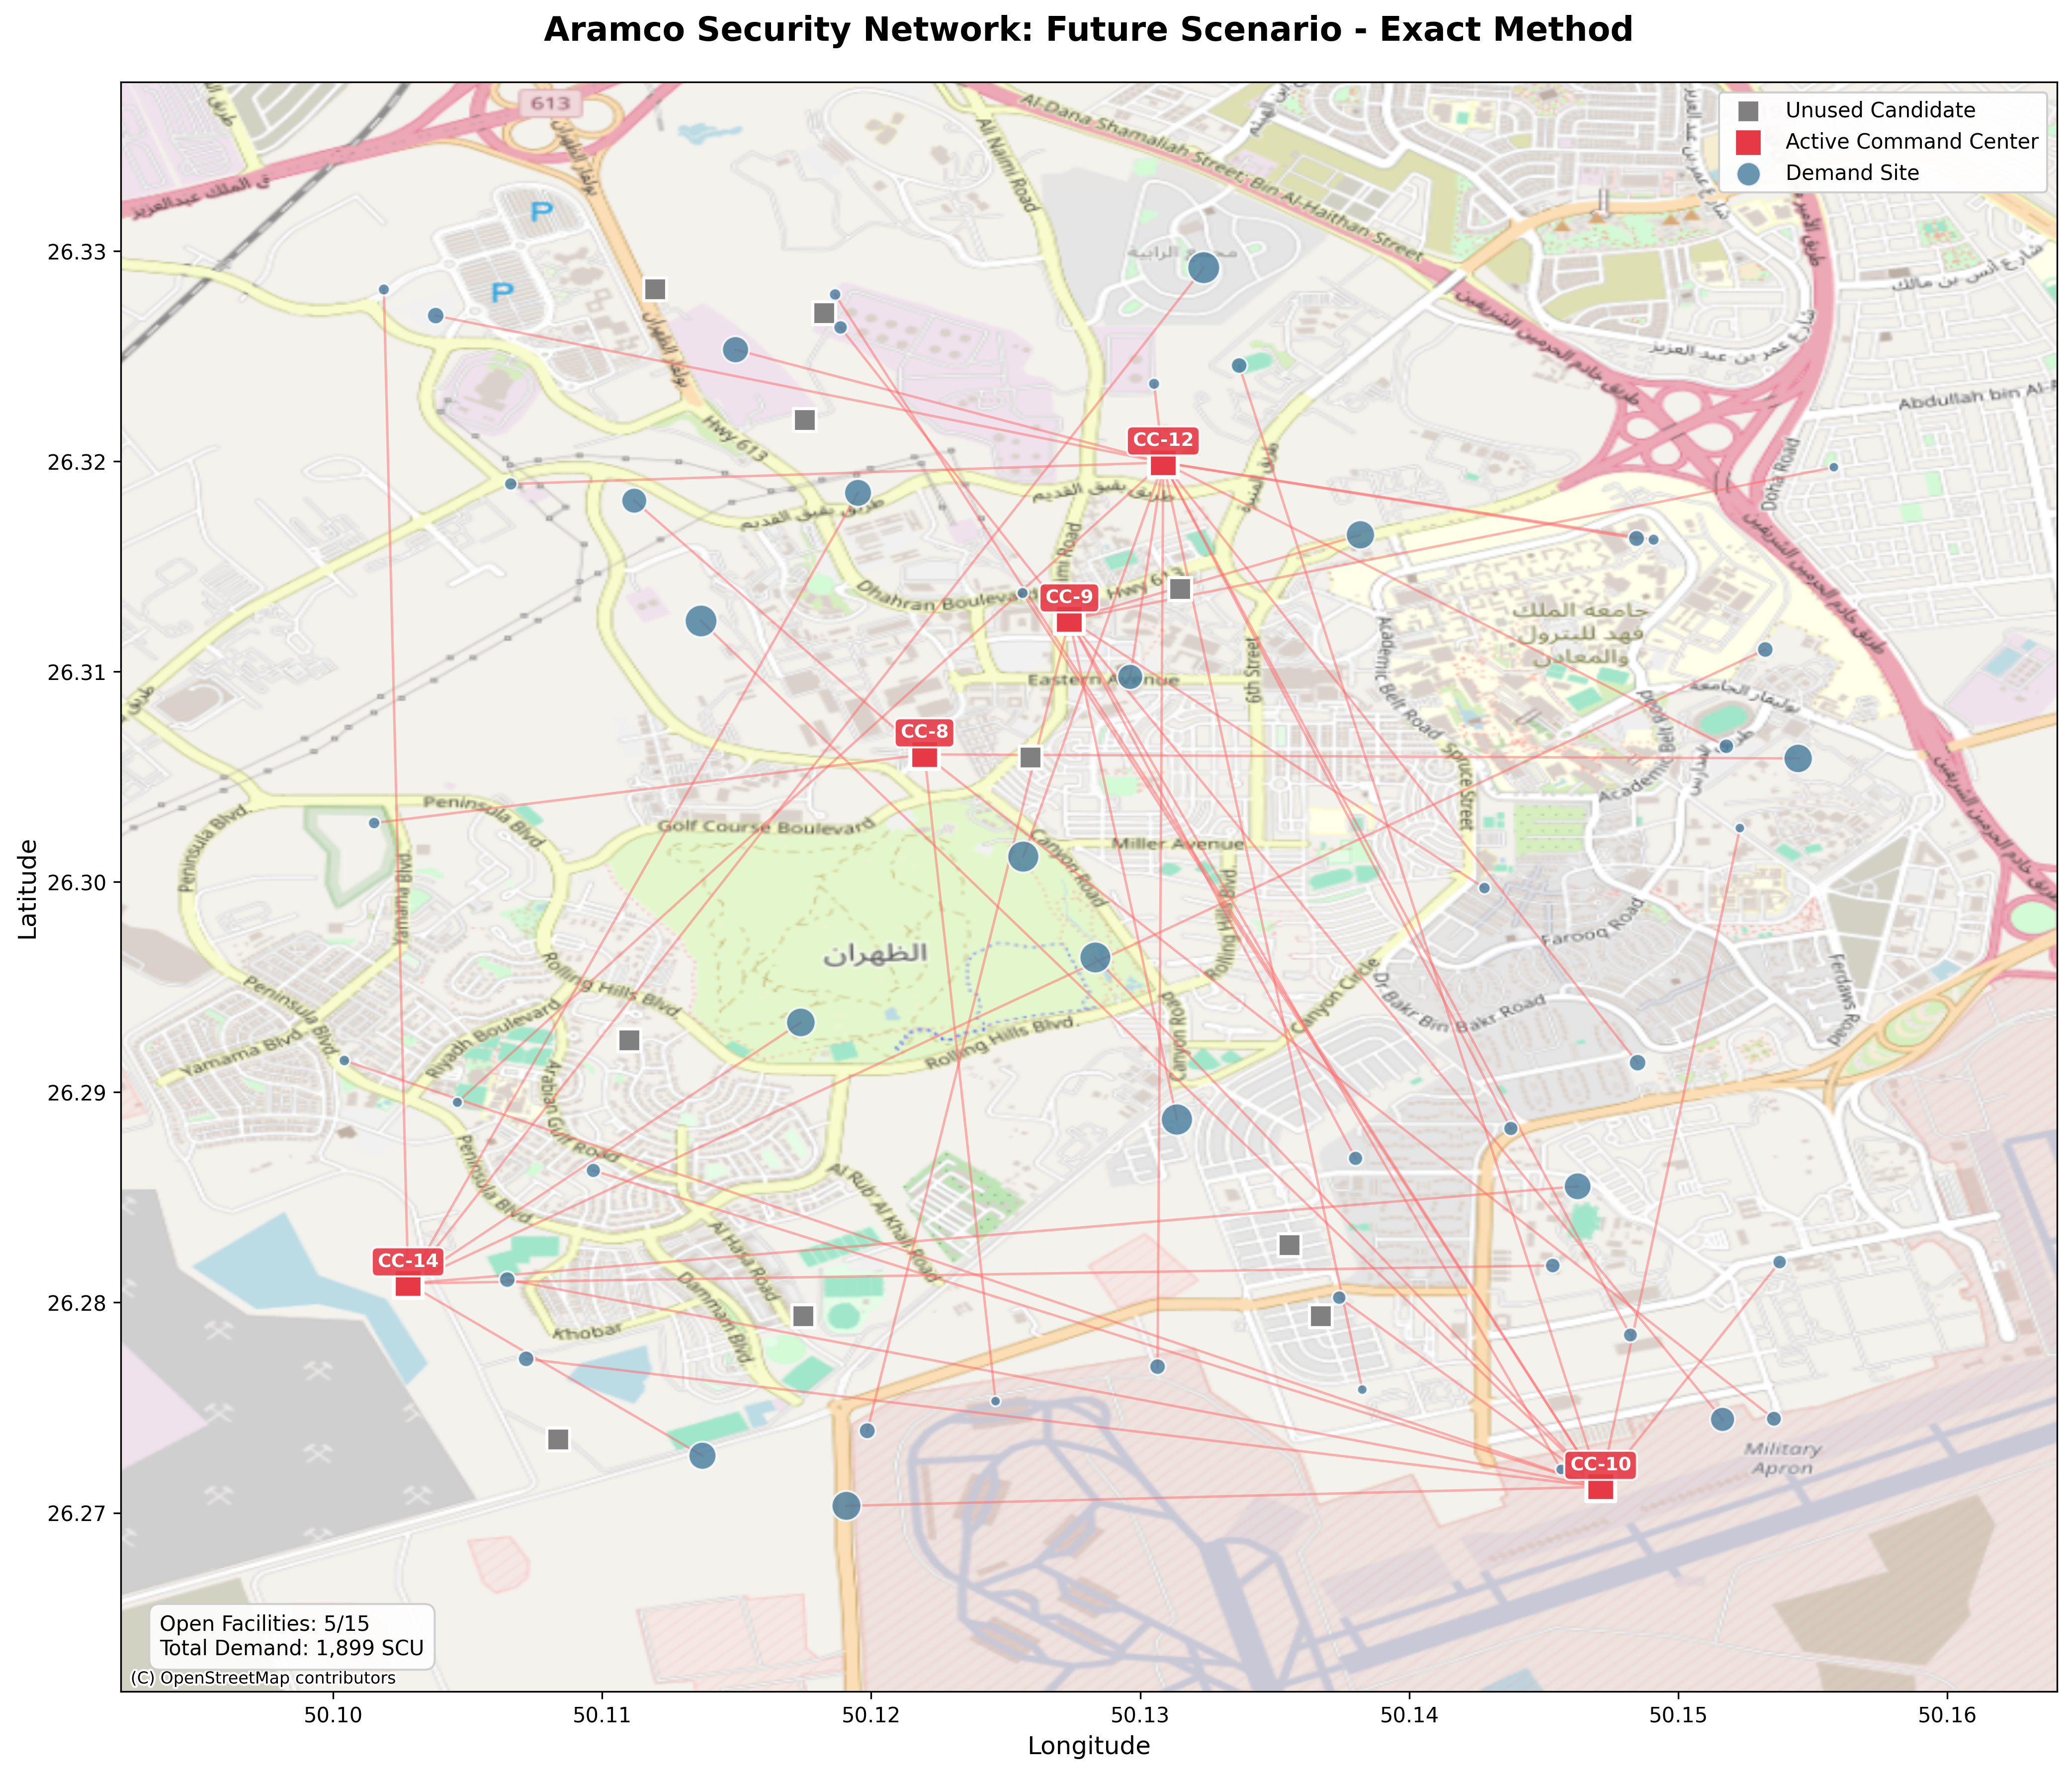
\includegraphics[width=0.85\textwidth]{figures/result_future_scenario_-_exact_method.pdf}
\caption{Future Scenario: Only 5 facilities required with advanced automation (1:10 supervision, 5x robot efficiency), demonstrating significant infrastructure consolidation potential.}
\label{fig:future}
\end{figure}

\subsection{Executable Deployment Plan}
Based on the Balanced (Current Technology) scenario, we present an executable deployment plan for the Dhahran district:

\textbf{Phase 1 - Infrastructure (Months 1-6):}
\begin{enumerate}
    \item Construct 7 command centers at optimal locations identified by the model.
    \item Prioritize locations 8-14 (peripheral sites) which serve the majority of demand.
    \item Total construction investment: \$140,000 (7 × \$20,000 average).
\end{enumerate}

\textbf{Phase 2 - Resource Deployment (Months 7-12):}
\begin{enumerate}
    \item Deploy robotic units (drones/UGVs) at each command center.
    \item Hire and train human supervisors at 1:5 ratio.
    \item Monthly operational cost: \$739,600 (\$879,600 - \$140,000 fixed).
\end{enumerate}

\textbf{Phase 3 - Technology Migration (Years 2-5):}
\begin{enumerate}
    \item Gradually transition toward Future scenario as AI maturity improves.
    \item Consolidate from 7 to 5 facilities, closing underutilized centers.
    \item Target monthly savings: \$367,200 (Balanced to Future difference).
\end{enumerate}

\subsection{Economic Impact Analysis}
Compared to a hypothetical baseline of full human deployment (without robotic augmentation), the proposed solutions offer substantial savings:

\begin{itemize}
    \item \textbf{Conservative Scenario:} Estimated 25\% savings vs. all-human baseline.
    \item \textbf{Balanced Scenario:} Estimated 45\% savings vs. all-human baseline.
    \item \textbf{Future Scenario:} Estimated 65\% savings vs. all-human baseline.
\end{itemize}

These projections assume a fully human-staffed baseline monthly cost of approximately \$1,800,000 (based on Tier 1 security personnel costs in the Eastern Province).

\section{Conclusions}
This study formulated and solved a Capacitated Facility Location Problem tailored for security command center optimization at Saudi Aramco's Dhahran headquarters. The mathematical model successfully integrates multiple real-world constraints including SLA compliance, human-robot supervision ratios, facility capacity limits, and minimum utilization requirements.

\subsection{Key Contributions}
\begin{enumerate}
    \item \textbf{Novel Problem Formulation:} We adapted the classical CFLP framework to explicitly model the trade-off between human security personnel and autonomous robotic units, incorporating supervision constraints unique to industrial security applications.
    
    \item \textbf{Computational Framework:} We developed a hybrid solution approach combining exact optimization (Gurobi) for benchmark solutions with a constructive greedy heuristic enhanced by Shift, Swap, and Drop/Open local search moves. The heuristic achieves less than 2.5\% optimality gap while running 10x faster.
    
    \item \textbf{Scenario Analysis:} By varying technological maturity parameters while keeping geography constant, we quantified the potential cost savings from automation: up to 63.4\% reduction when transitioning from conservative to fully autonomous operations.
    
    \item \textbf{Deployment Roadmap:} The executable deployment plan provides Saudi Aramco with a phased approach to implement the optimal solution, starting with current technology and evolving toward higher automation as AI capabilities mature.
\end{enumerate}

\subsection{Limitations}
\begin{itemize}
    \item \textbf{Synthetic Data:} While coordinates are based on the real Dhahran topology, specific demand values and cost parameters were synthetically generated based on industry estimates rather than actual Aramco operational data.
    \item \textbf{Static Model:} The current formulation assumes static demand; future work could incorporate time-varying demand patterns (day/night shifts, seasonal variations).
    \item \textbf{Single-Period Planning:} The model optimizes a single planning period; multi-period capacity expansion models could capture facility construction sequencing more accurately.
\end{itemize}

\subsection{Future Research Directions}
\begin{enumerate}
    \item \textbf{Stochastic Demand:} Incorporate uncertainty in security demand using robust or chance-constrained optimization.
    \item \textbf{Dynamic Response Modeling:} Add explicit travel time modeling with routing constraints rather than simple SLA distance limits.
    \item \textbf{Multi-Objective Optimization:} Balance cost minimization against response time minimization and coverage maximization using Pareto-optimal frontiers.
    \item \textbf{Real-World Validation:} Collaborate with Saudi Aramco to validate the model using actual operational data and conduct pilot deployments.
    \item \textbf{Integration with IoT:} Extend the framework to incorporate real-time sensor data for adaptive resource reallocation.
\end{enumerate}

\subsection{Final Remarks}
The optimization framework developed in this study demonstrates that significant operational cost savings are achievable through strategic facility location and human-robot resource allocation. As autonomous security technologies continue to mature, organizations like Saudi Aramco can leverage such decision-support tools to systematically plan their transition toward Industry 4.0 security operations while maintaining the human oversight essential for ethical and effective decision-making. Source code available at: \url{https://github.com/naimackerman/aramco_security_opt}

\end{document}